\documentclass[aps, pra, 10pt, twocolumn, superscriptaddress,floatfix]{revtex4-1}

\usepackage{amsmath,amssymb,amsfonts}
\usepackage{braket}
\usepackage[breaklinks=true,colorlinks,citecolor=blue,linkcolor=blue,urlcolor=blue]{hyperref}
\usepackage{mathtools}
\usepackage{dsfont}

%%
\def \id {\mathds{1}}
\def \abs {\text{Abs}}
\newcommand{\norm}[1]{\lVert#1\rVert}
\DeclareMathOperator{\tr}{Tr}
\newcommand{\round}[1]{\ensuremath{\lfloor#1\rceil}}
\newcommand{\mi}{\mathrm{i}} %% roman "i"
%

\begin{abstract}
	In a previous work we have been using an optical platform to test an offline metrological protocol for the estimation of a rotation angle at the Heisenberg scaling. In this notes we deal with the two problems of estimating a phase on the same setup when the visibilities are unknown and are treated as \textit{nuisance} parameters, and the problem of determining one ore more visibilities of the optical components (q-plates) of the setup together with the rotation angle. Finally, with the estimation of all the parameters we perform a characterization of the whole system. We confront the estimated MSE, obtained with $50$ repetitions of each experiments with the van Trees bound (the Bayesian Cramer-Rao bound).
\end{abstract}

\begin{document}
%
\title{Characterization of a metrological optical setup with nuisance parameters} 
%
\author{Federico Belliardo}
\email{federico.belliardo@sns.it}
\affiliation{NEST, Scuola Normale Superiore, I-56126 Pisa,~Italy}

\maketitle


\section{Introduction}
%
In this work we want to study the complete characterization of an optical setup, that might be later used by the experimentalists to carry out quantum protocols. We are going to employ the q-plate setup of~\cite{Cimini2021}, see Fig.~\ref{fig:apparatus}, with three q-plates. This means the apparatus will be characterized by four visibilities: one for the configuration without active q-plates and three for the three configurations with only one q-plate active each. 
%
\begin{figure}[!th]
	\begin{center}
		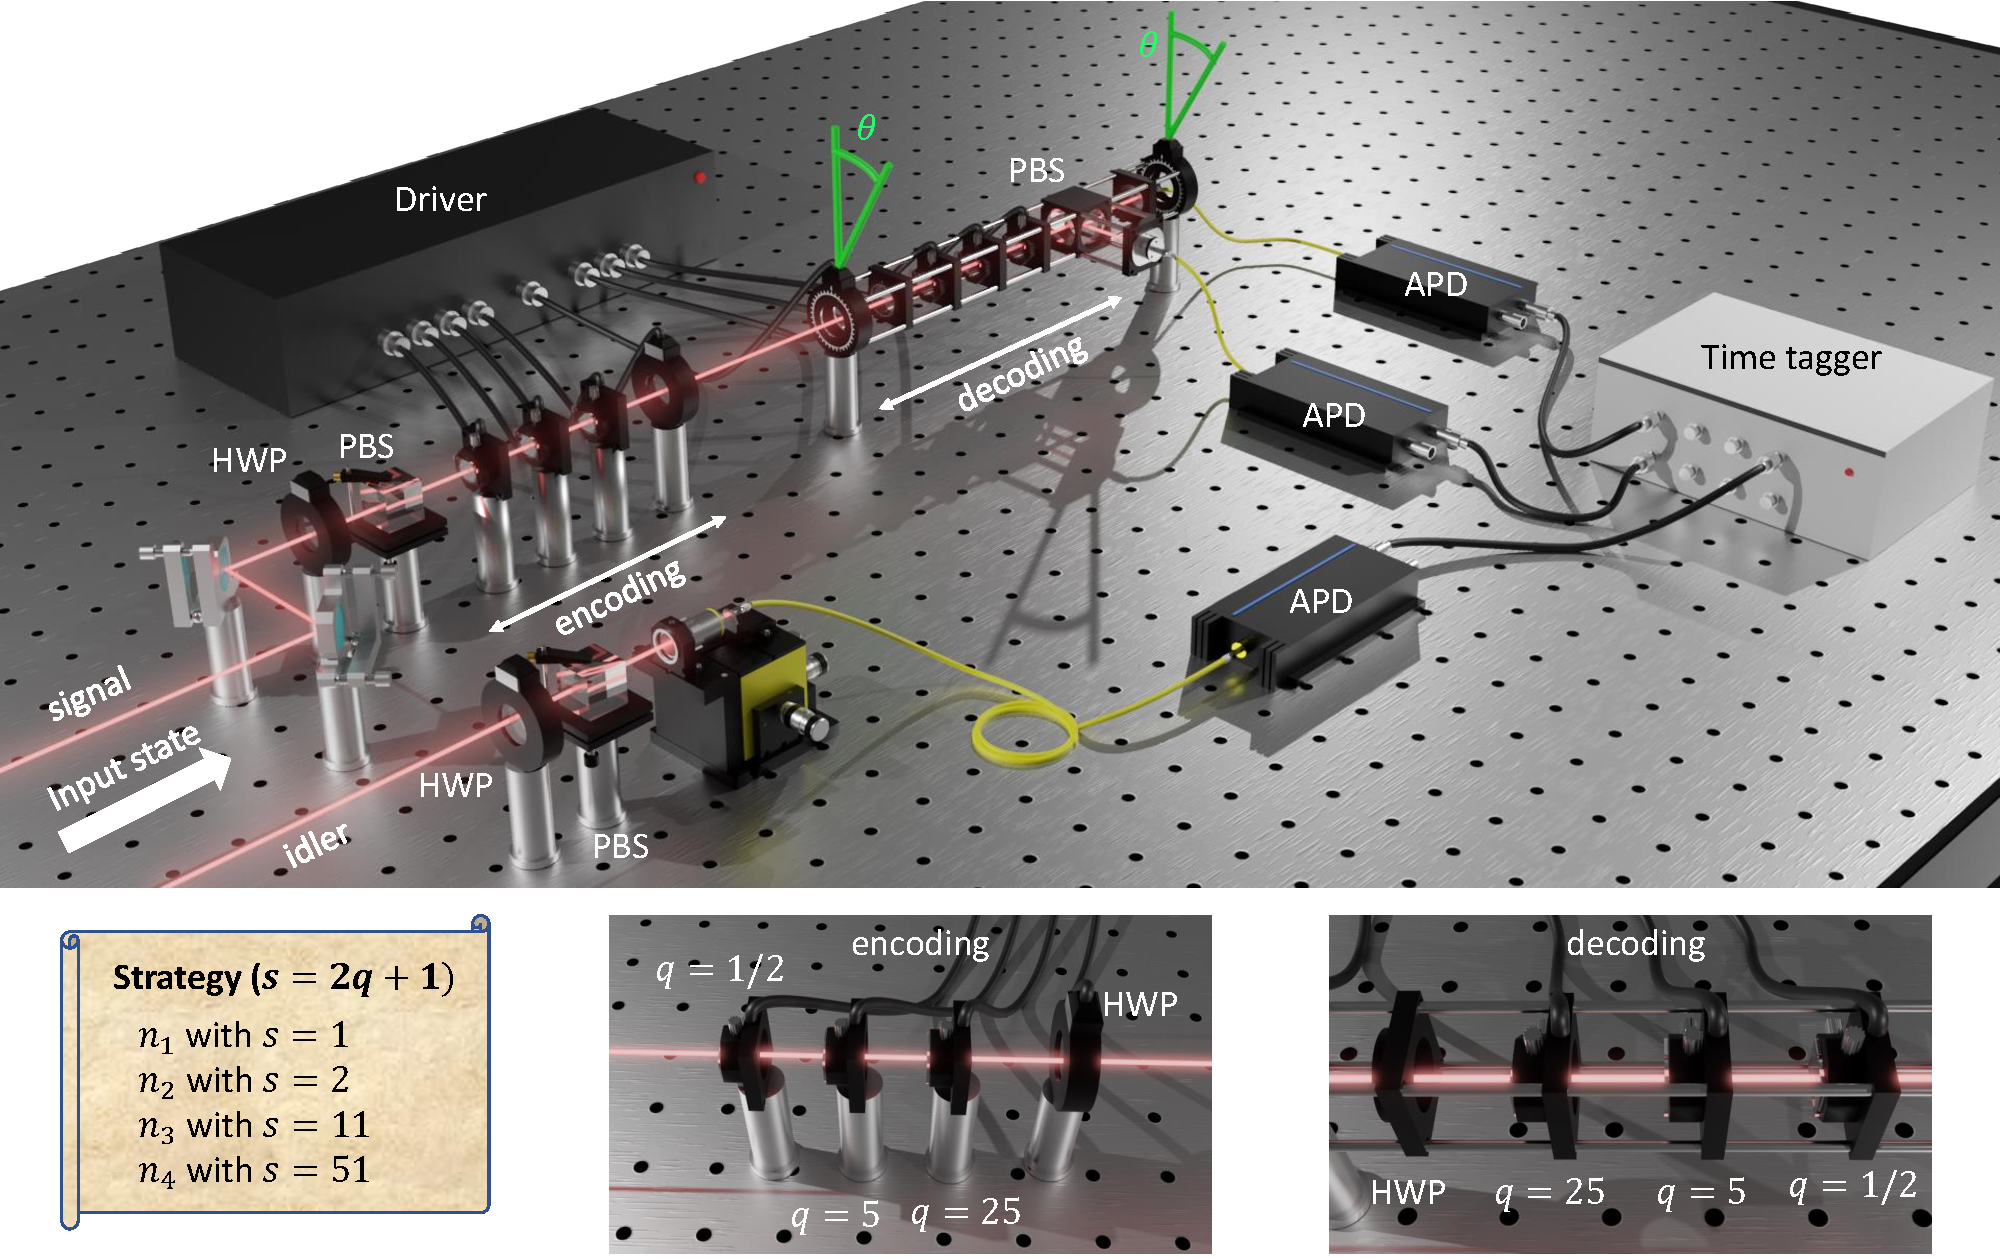
\includegraphics[width=0.5\textwidth]{FigureSetup.pdf}
	\end{center}
	\caption{View of the experimental apparatus with the three q-plates.}
	\label{fig:apparatus}
\end{figure}
%
Therefore the parameters to estimate are a rotation angle $\theta \in [0, \pi)$ and the four visibilities $V_1, V_2, V_3, V_4 \in [0, 1]$. In all the Bayesian experiments performed here the prior distributions on the visibilities will be uniform in $[0, 1]$. The Bayesian procedure will be implemented as presented in~\cite{Granade2012} with a particle filter. This method selects the next measurement to be done (the next q-plate) according to the posterior probability distribution for the unknown phase and visibilities. We will first measure only the phase $\theta$ treating the visibilities as \textit{nuisance} parameters. That means our goal will first be the minimization of the mean square error on the phase only. Here the estimators for the visibilities should be only precise enough to allow us to find a good strategy for the estimation of the phase. Then we will minimize the error on a couple of parameters, that is the phase and one of the visibilities: $(\theta, V_i)$ with $i=1, 2, 3, 4$, the other three visibilities will be again nuisance parameters. At the end we try to estimate all the five parameters $(\theta, V_1, V_2, V_3, V_4)$ at the same time. 

\section{The Bayesian procedure}
%
In this section we present the Bayesian algorithm proposed in~\cite{Granade2012}, with the application to our q-plates setup in mind. With respect to the original formulation we made a few corrections necessary because of the circular nature of the angular variable that we are going to measure. In every simulated experiment $n_p = 1000$ particles have been used. The parameters to estimate are collected in the vector $\boldsymbol{x} := \left( \theta, V_1, V_2, V_3, V_4 \right)$, that contains the phase in the first entry and the four visibilities in the other ones. Being the Granade's method based on a particle filter, it represents internally the posterior probability distribution with the ensemble $\mathcal{E} := \lbrace \boldsymbol{x}^i, w^i \rbrace$, where $\boldsymbol{x}^i$ is the position of the $i$-th particle and $w^i$ its weight. The $j$-th component of the $i$-th particle of the ensemble will be represented as $x_j^i$, and could correspond to the phase if $j=0$, that is $x^i_0 = \theta^i$ or to one of the visibilities if $j=1, 2, 3, 4$, that is $x^i_j = V^i_j$. The mean of the angular values is computed as
%
\begin{equation}
	\hat{\mu}_0 := \arg \left[ \sum_{i=1}^{n_{p}} w^i \exp \left( \mi \theta^i \right) \right] \; ,
\end{equation}
%
while the mean values of the visibilities are
%
\begin{equation}
	\hat{\mu}_j = \sum_{i=1}^{n_p} w^i V^i_j \; .
\end{equation}
%
Together they form the vectorial mean of the distribution $\boldsymbol{\hat{\mu}} = (\hat{\mu}_0, \hat{\mu}_1, \hat{\mu}_2, \hat{\mu}_3, \hat{\mu}_4)$. The covariance matrix is defined as
%
\begin{equation}
	\text{Cov}_{ij} := \sum_{k=1}^{n_{p}} w^k (x^k_i - \hat{\mu}_i)  (x^k_j - \hat{\mu}_j) \; .
\end{equation}
%
If $i=1$ or $j=1$ then difference in $x^k_i - \hat{\mu}_i$ or $x^k_j - \hat{\mu}_j$ is actually the circular distance
%
\begin{equation}
	d(x^k_i, \hat{\mu}_i) = \pi - | (x^k_i - \hat{\mu}_i) \mod 2 \pi - \pi| \; .
\end{equation}
%
The Bayesian algorithm tries for each new experiment (each new photon sent with a specific q-plate activated) to minimize the scalar variance of the posterior distribution, that is
%
\begin{equation}
	\sigma^2 := \tr \left[ G \cdot \text{Cov} \right] = \sum_{i, j} G_{ij} \text{Cov}_{ij} \; ,
\end{equation}
%
where $G$ is the weight matrix that controls which parameters are to be treated as nuisance parameters. In this way the algorithm attempts to concentrate as much as possible the distribution around its mean in a greedy fashion. In the plots of Sec.~\ref{sec:results} we reported the MSE, which is computed repeating $50$ times each experiment for a given rotation angle and total resource number. The resampling strategy of the Granade procedure has also undergone minor changes to adapt it to the phase estimation problem. We have performed only simulations (we didn't use the actual experimental data collected) with visibilities $V_1 = 0.900$, $V_2 = 0.875$, $V_3 = 0.850$ and $V_4 = 0.765$, for $17$ angles chosen in $[0, \pi)$ that have been measured in the actual experiment. At difference with the offline algorithm we can't perform the estimation with a fixed number $N$ of total used resources, because the number of photons to use for each q-plate is a stochastic variable, this makes $N$ a stochastic variable too. Only the total number of used photons can be fixed.  In the rest of this section we will refer to the estimation of the rotation angle only, that is the MSE will be $\Delta^2 \hat{\theta}$. If two or more parameters are to be evaluated the MSE of the angle should be substituted with the sum of the errors, e.g. $\Delta^2 \hat{\theta} + \Delta^2 \hat{V}$. In order to give a synthetic representation of the performances of the Bayesian method we proceed as following. We perform $50$ estimations for each of the angles with a total number of resources $N=30000$, and we save for each new photon measurement the estimators $\hat{\theta}$, $\hat{V}_j$ and the total number of used resources $N$ up to that point. For a certain angle, we consider all the $n$ measurements with resources falling in $[N, N+\Delta N]$ as if they were performed with the same resource number and use them to compute the MSE. For each angle $\theta_j$, indexed with $j=1, \dots, J$, the error is
%
\begin{equation}
	\Delta^2 \hat{\theta}_j = \frac{1}{n} \sum \limits_{k=1}^{n} | \hat{\theta}_{jk} - \theta_j |^2 \; .
\end{equation}
%
We compute the square root of the variance of $| \hat{\theta}_{jk} - \theta_j |^2$, and the error on the mean is
%
\begin{equation}
	\delta \Delta^2 \hat{\theta}_j = \frac{ \sigma \left( | \hat{\theta}_j - \theta_j |^2 \right)}{\sqrt{n}} \; ,
\end{equation}
%
with 
%
\begin{equation}
\sigma \left( | \hat{\theta}_j - \theta_j |^2 \right) := \sqrt{\frac{\sum \limits_{k=1}^{n} | \hat{\theta}_{jk} - \theta_j |^4}{n} - \left( \frac{\sum \limits_{k=1}^{n} | \hat{\theta}_{jk} - \theta_j |^2 }{n} \right)^2} \; .
\end{equation}
%
In the plots we visualize the mean MSE for the $J=17$ angles, i.e.
%
\begin{equation}
\overline{\Delta^2 \hat{\theta}} = \frac{1}{J} \sum \limits_{j=1}^{J} \Delta^2 \hat{\theta}_j \; .
\end{equation}
%
The error (square root of the variance) of this mean will be
%
\begin{equation}
	\delta \overline{\Delta^2 \hat{\theta}} = \frac{1}{J} \sqrt{ \sum \limits_{j=1}^{J} \left( \delta \Delta^2 \hat{\theta}_j \right)^2}\; .
\label{eq:errory}
\end{equation}
%
Using this procedure means that the resources consumed for each point has a certain dispersion, that becomes the x-axis error in the plots of Sec.~\ref{sec:results}. The value of $\Delta N$ changes according to $N$, in particular we have $\Delta N = 2$ for $N \in \left[2, 100 \right]$, $N = 20$ for $N \in \left[100, 1000 \right]$ and $\Delta N = 50$ for $N \in \left[1000, 30000 \right]$. 

\section{The van Trees bound}
%

Consider $\nu$ repetitions of a couple of Type-$0$ and Type-$+$ measurements~\cite{Belliardo2020} performed with a certain q-plate of charge $s$, that produce two results $c_1, c_2 \in \lbrace -1, +1 \rbrace$ each, extracted from the following two probability distribution
%
\begin{equation}
	p_1(c_1; \theta, V) = \frac{1 + c_1 \cdot V \cos s \theta}{2} \; ,
\end{equation}
%
and 
%
\begin{equation}
	p_2(c_2; \theta, V) = \frac{1 + c_2 \cdot V \sin s \theta}{2} \; .
\end{equation}
%
Our goal is to bound the precision of the joint estimation of $V$ and $\theta$. With this goal we compute the Fisher information matrix for the estimation of this couple of parameters for a pair of Type-$0$ and Type-$+$ measurements, which we call respectively $I_0 (\theta, V)$ and $I_+ (\theta, V)$, and sum them to get $I(\theta, V) := I_0 (\theta, V) + I_+ (\theta, V)$. We obtain the total Fisher information matrix for the angle and the visibilities of all the q-plates by summing the FI matrices corresponding to each quantum resource $s$, for a number $\nu_i$ of couple of measurements respectively. It is important that we think $I_i (\theta, V_i)$ as a $5 \times 5$ matrix even if only four entries for each matrix will be non null. In this way we can write the $5 \times 5$ FI matrix for the five parameters $(\theta, V_1, V_2, V_3, V_4)$ as
%
\begin{equation}
	I(\theta, V_1, V_2, V_3, V_4) := \sum_{i=1}^4 \nu_i I_i (\theta, V_i) \; .
\end{equation}
%
We report in the following all the non-zero entries of this matrix.
%
\begin{align}
		I(1, 1) &= \sum_{i=1}^4 \frac{2 s_i^2 V_i^2 \nu_i \left( -4 + 3 V_i^2 + V_i^2 \cos 4 s_i \theta \right)}{-8 + 8 V_i^2 -V_i^4 +V_i^4 \cos 4 s_i \theta} \; ,\\
		I(1, 2) &= I(2, 1) = -\frac{2 s_1 V_1^3 \nu_1 \cot 2 s_1 \theta}{(V_1^2 - \csc ^2 s_1 \theta)(V_1^2 -\sec ^2 s_1 \theta)} \; , \\
		I(1, 3) &= I(3, 1) = -\frac{2 s_2 V_2^3 \nu_2 \cot 2 s_2 \theta}{(V_2^2 - \csc ^2 s_2 \theta)(V_2^2 -\sec ^2 s_2 \theta)} \; , \\
		I(1, 4) &= I(4, 1) = -\frac{2 s_3 V_3^3 \nu_3 \cot 2 s_3 \theta}{(V_3^2 - \csc ^2 s_3 \theta)(V_3^2 -\sec ^2 s_3 \theta)} \; , \\
		I(1, 5) &= I(5, 1) = -\frac{2 s_4 V_4^3 \nu_4 \cot 2 s_4 \theta}{(V_4^2 - \csc ^2 s_4 \theta)(V_4^2 -\sec ^2 s_4 \theta)} \; , \\
		I(2, 2) &= \nu_1 \left( \frac{1}{-V_1^2 + \csc^2 s_1 \theta} + \frac{1}{-V_1^2 + \sec^2 s_1 \theta}\right) \; ,\\
		I(3, 3) &= \nu_2 \left( \frac{1}{-V_2^2 + \csc^2 s_2 \theta} + \frac{1}{-V_2^2 + \sec^2 s_2 \theta}\right) \; ,\\
		I(4, 4) &= \nu_3 \left( \frac{1}{-V_3^2 + \csc^2 s_3 \theta} + \frac{1}{-V_3^2 + \sec^2 s_3 \theta}\right) \; ,\\
		I(5, 5) &= \nu_4 \left( \frac{1}{-V_4^2 + \csc^2 s_4 \theta} + \frac{1}{-V_4^2 + \sec^2 s_4 \theta}\right) \; ,
\end{align}
%

We now introduce a Bayesian version of the Cramer-Rao bound, called the van Trees bound. Consider the Bayesian estimation of a vector of parameters $\boldsymbol{x} = (x_1, x_2, \cdots, x_K)$ with prior $\pi (\boldsymbol{x})$, then the expectation values of the MSE matrix can be bounded as following
%
\begin{equation}
	\mathbb{E}_\pi \left[ \mathbb{E} \left[ (\boldsymbol{x} - \boldsymbol{x}_0)^T  (\boldsymbol{x} - \boldsymbol{x}_0) \right] \right] \ge \left( \mathbb{E}_\pi [I(\boldsymbol{x})] + I_\pi \right)^{-1} \; .
\end{equation}
%
In this expression $I_\pi$ is the Fisher information associated to the prior distribution. In our case the prior is uniform and doesn't carry any information, therefore $I_\pi = 0$. We compute the expectation value in $\theta$ of the Fisher information $I(\theta, V_1, V_2, V_3, V_4)$ and obtain a diagonal expression, with entries
%
\begin{equation}
	\mathbb{E}_\pi [ I](1, 1) = 2 \sum_{i=1}^4 \nu_i s_i^2 \left( 1 - \sqrt{1-V_i^2}\right) \; ,
\end{equation}
%
\begin{equation}
	\mathbb{E}_\pi [ I] (i+1, i+1) = \frac{2 \nu_i \left( 1 - \sqrt{1-V_i^2} \right)}{V_i^2 \sqrt{1-V_i^2}}\, , \text{for} \; i=1, \dots, 4 \; .
\end{equation}
%
We can give a lower bound on the average MSE via the following non-linear program
%
\begin{equation}
    \begin{cases}
	\min \tr \left( G \cdot \mathbb{E}_\pi [ I]^{-1} \right)\\
	\text{subject to} \; 2 \sum_{i=1}^4 s_i \nu_i = N \\
	\nu_i \ge 0 
	\end{cases}\\
	\; .
	\label{eq:semidefinite}
\end{equation}
%
The solution of such non-linear minimization gives a lower bound on the expected MSE of the form 
%
\begin{equation}
	\mathbb{E}_\pi \left[ \mathbb{E} \left[ (\boldsymbol{x} - \boldsymbol{x}_0)^T  (\boldsymbol{x} - \boldsymbol{x}_0) \right] \right] \ge \frac{C}{N} \; .
	\label{eq:vanTrees}
\end{equation}
%
The constant $C$ can be determined by solving the non-linear program
%
\begin{equation}
	 \begin{cases}
	\min \tr \left( G \cdot \mathbb{E}_\pi [ I]^{-1} \right)\\
	\text{subject to} \; 2 \sum_{i=1}^4 s_i \nu_i = 1 \\
	\nu_i \ge 0 
	\end{cases}\\
	\; .
\end{equation}
%
The van Trees bound in Eq.~\eqref{eq:vanTrees} is the green line in the plots of Sec.~\ref{sec:results}, and is valid only asymptotically. The mean value of the MSE on all the $J=17$ angles is an approximation of the expectation value of the MSE on the uniform prior $\pi$ (in $\theta$), i.e. $\mathbb{E}_\pi [\Delta^2 \hat{\theta} ]$. In the plots we want to combine the information of many experiments performed with different phases, therefore we need to compare the data with bounds independent on $\theta$, for this reason we introduced the expectation value on $\theta$. {\color{red} In this Bayesian approach I should have taken also the average on $V_i$.}


\section{Results of the simulations}
\label{sec:results}
%
In this section we report the simulated MSE compared with the theoretical bound in Eq.~\eqref{eq:vanTrees}. First of all in Fig.~\ref{fig:theta} the precision for the estimation of the rotation angle only is showed, here all the visibilities are treated as nuisance parameters. In Fig.~\ref{fig:thetaV1}, \ref{fig:thetaV2}, \ref{fig:thetaV3}, \ref{fig:thetaV4} we report the precision of the estimation of two phases and a visibility.
%That is, the Bayesian algorithm seeks to minimize the variance of the posterior, and does so, however the small but non-null bias of the estimator prevents the MSE to decrease.
Fig.~\ref{fig:allParameters} contains the precision for the joint estimation of all the five parameters. The hump in plots~\ref{fig:thetaV3}, \ref{fig:thetaV4}, and Fig.~\ref{fig:allParameters} is due to the fact that only from a certain number of resources the Bayesian algorithm starts to use consistently the q-plate having the visibility we are interested in. 
%Up to that point the distribution of the estimator $\hat{V}_i$ remains uniform in $[0, 1]$ (the prior) and the MSE remains $\frac{1}{12} + (0.5-V_i)$, that is the variance of the uniform distribution plus the bias. Depending on the value of $s$ (the quantum resource) there might be a regime where the error $\Delta^2 \hat{\theta} + \Delta^2 \hat{\theta}$ converges to $\frac{1}{12} + (0.5-V_i)$. In the plots~\ref{fig:thetaV1}, \ref{fig:thetaV2}, \ref{fig:thetaV3}, \ref{fig:thetaV4} the yellow line is $\frac{1}{12} + (0.5-V_i)$.
The precision of all the visibilities saturates after a certain point, this might be related to the number of particles $n_p$ and to the hyperparameters of the Bayesian procedure. In Fig.~\ref{fig:thetaV2-5000} we report the results of the estimation of the couple $(\theta, V_2)$ with $n_p = 5000$, and indeed the precision seems improved. The purple line is the precision of the estimation. In blue we plot the error bars.
%
\begin{figure}[!th]
	\begin{center}
		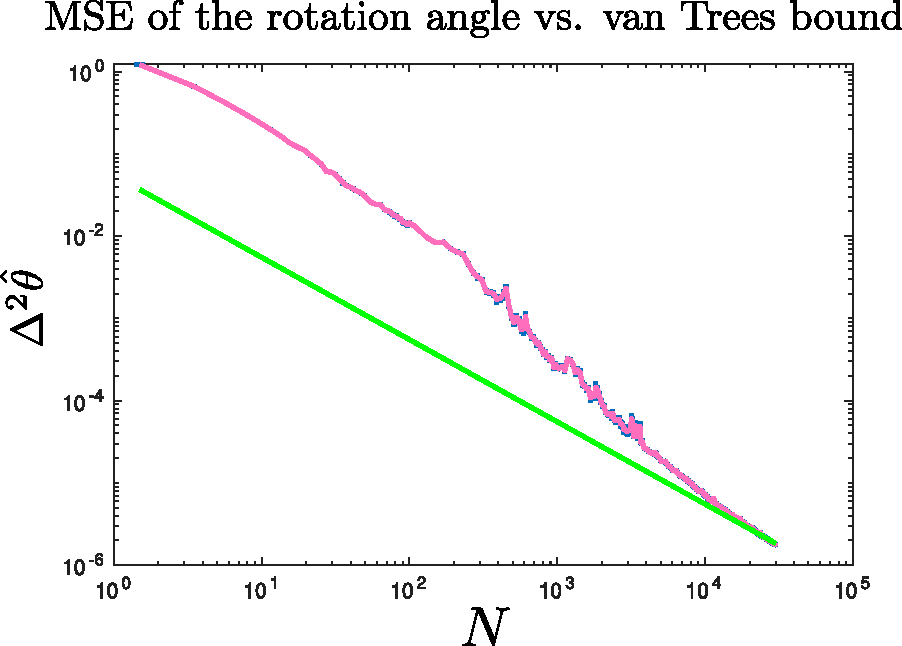
\includegraphics[width=0.5\textwidth]{theta.pdf}
	\end{center}
	\caption{Estimation of the rotation angle in which the visibilities are considered as nuisance parameters. The weight matrix has $G_{11} = 1$ as only non-null entry. The purple line is the precision of the estimation. In blue we plot the error bars.}
	\label{fig:theta}
\end{figure}
%
\begin{figure}[!t]
	\begin{center}
		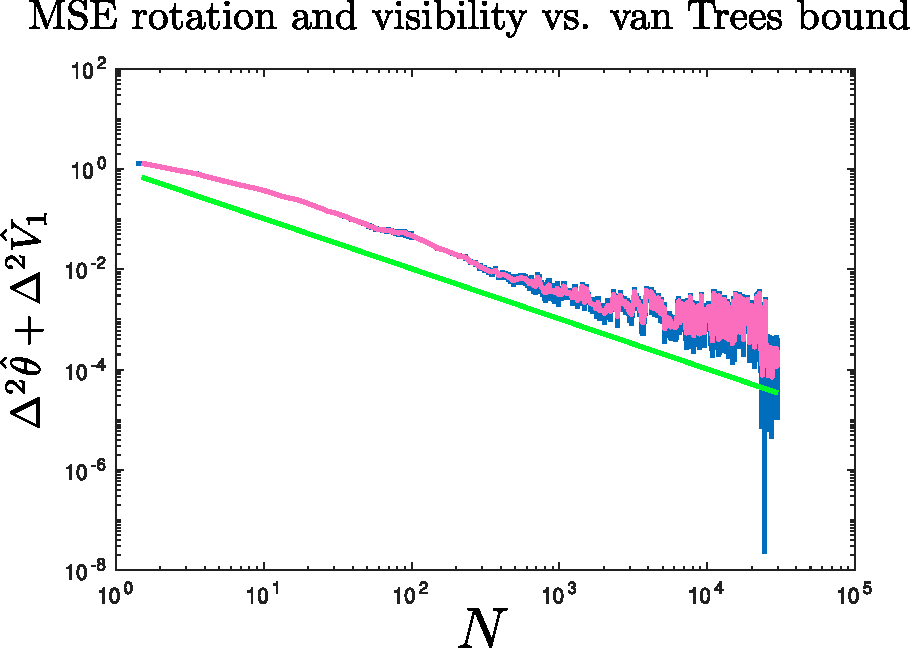
\includegraphics[width=0.5\textwidth]{thetaV1.pdf}
	\end{center}
	\caption{Estimation of the rotation angle and the first visibility (for all the q-plates switched off) in which the other visibilities are considered as nuisance parameters. The weight matrix has $G_{11} = 1$ and $G_{22} = 1$ as only non-null entries. The purple line is the precision of the estimation. In blue we plot the error bars.}
	\label{fig:thetaV1}
\end{figure}
%
\begin{figure}[!t]
	\begin{center}
		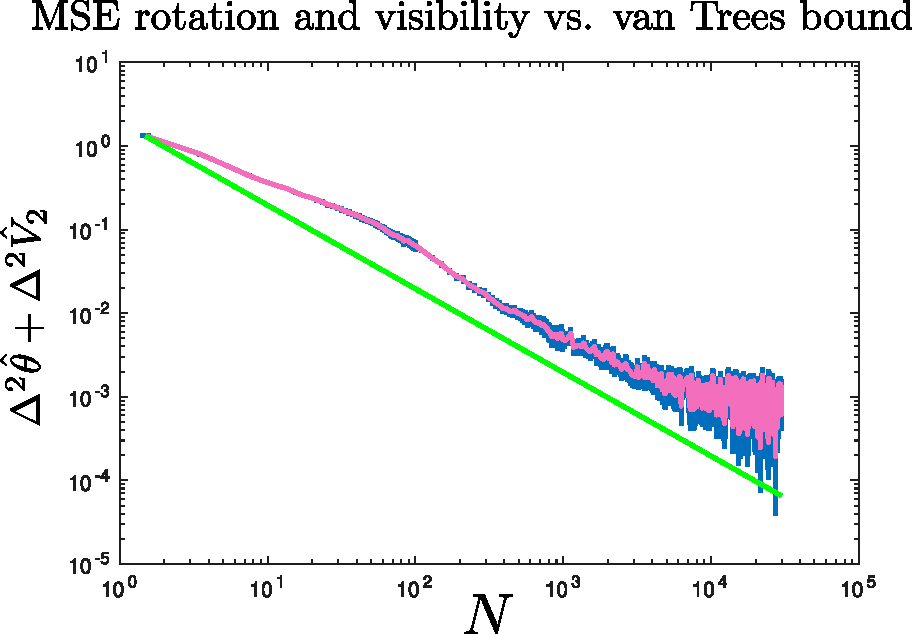
\includegraphics[width=0.5\textwidth]{thetaV2.pdf}
	\end{center}
	\caption{Estimation of the rotation angle and the second visibility (for the stage $s=2$) in which the other visibilities are considered as nuisance parameters. The weight matrix has $G_{11} = 1$ and $G_{33} = 1$ as only non-null entries. The purple line is the precision of the estimation. In blue we plot the error bars.}
	\label{fig:thetaV2}
\end{figure}
%
\begin{figure}[!t]
	\begin{center}
		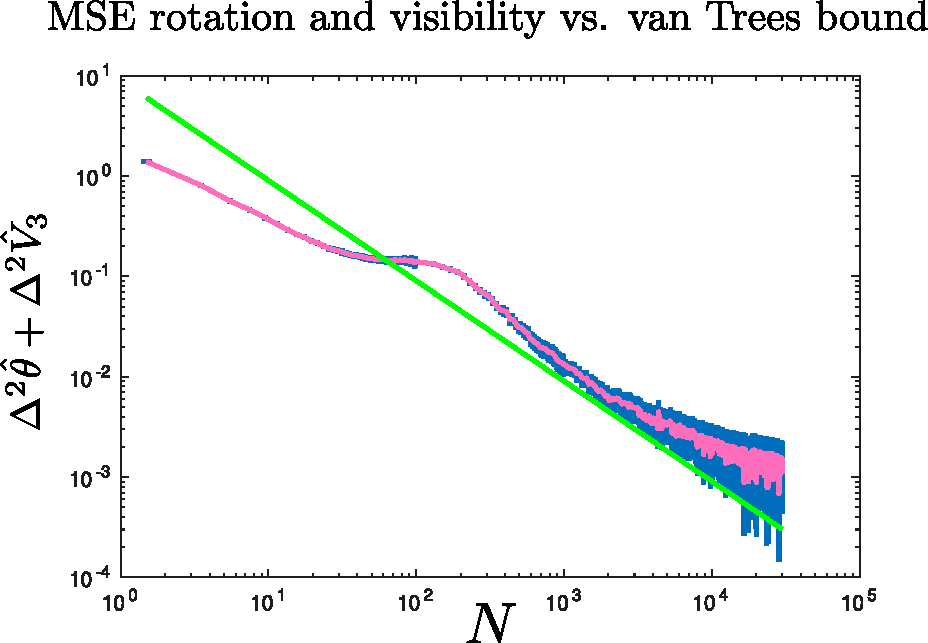
\includegraphics[width=0.5\textwidth]{thetaV3.pdf}
	\end{center}
	\caption{Estimation of the rotation angle and the third visibility (for the stage $s=11$) in which the other visibilities are considered as nuisance parameters. The weight matrix has $G_{11} = 1$ and $G_{44} = 1$ as only non-null entries. The purple line is the precision of the estimation. In blue we plot the error bars.}
	\label{fig:thetaV3}
\end{figure}
%
\begin{figure}[!t]
	\begin{center}
		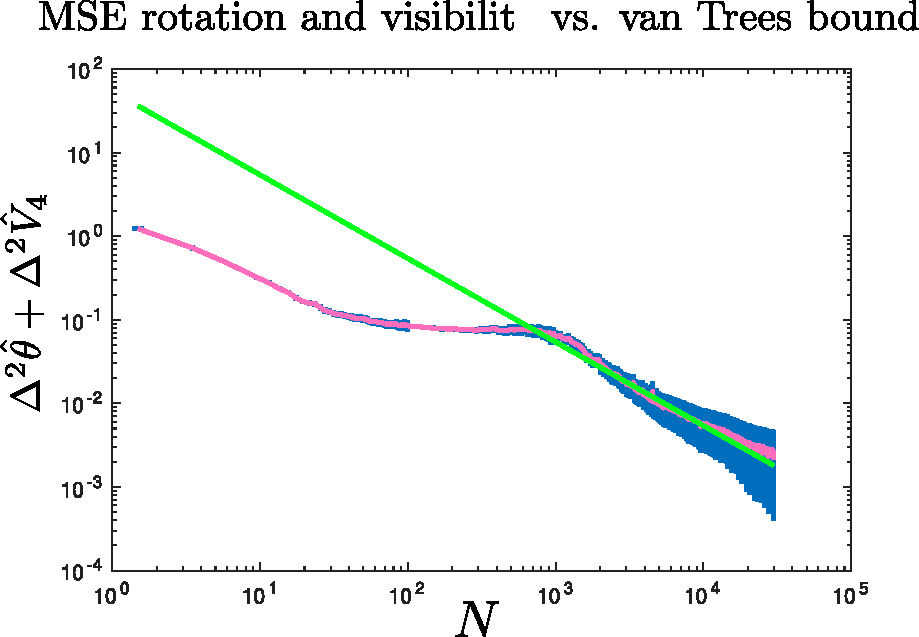
\includegraphics[width=0.5\textwidth]{thetaV4.pdf}
	\end{center}
	\caption{Estimation of the rotation angle and the forth visibility (for the stage $s=51$) in which the other visibilities are considered as nuisance parameters. The weight matrix has $G_{11} = 1$ and $G_{55} = 1$ as only non-null entries. The purple line is the precision of the estimation. In blue we plot the error bars.}
	\label{fig:thetaV4}
\end{figure}
%
\begin{figure}[!t]
	\begin{center}
		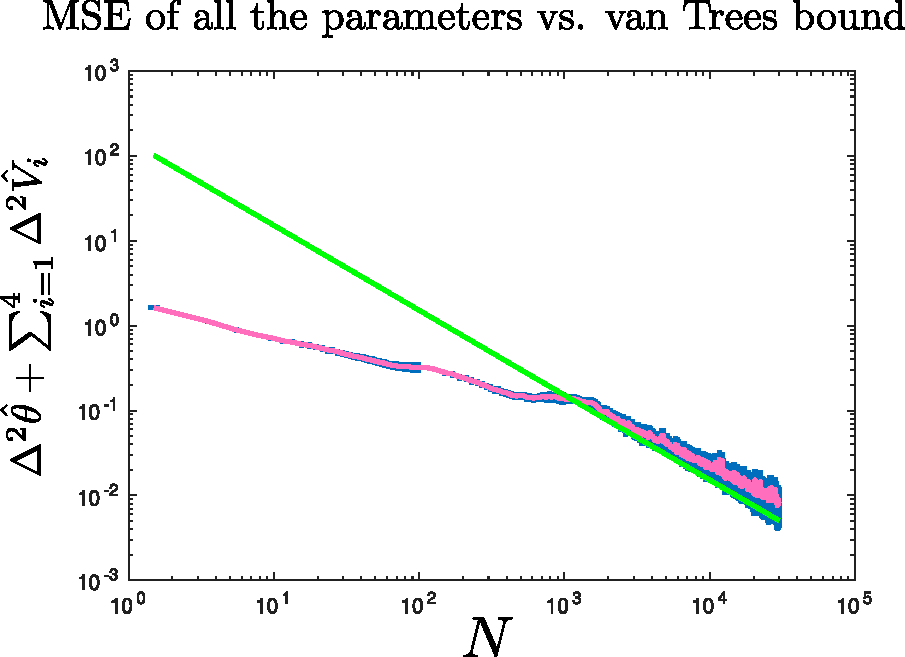
\includegraphics[width=0.5\textwidth]{multiparameter.pdf}
	\end{center}
	\caption{Estimation of the rotation angle and all the for visibilities jointly. The weight matrix is $G = \id$. The purple line is the precision of the estimation. In blue we plot the error bars.}
	\label{fig:allParameters}
\end{figure}
% 
\begin{figure}[!t]
	\begin{center}
		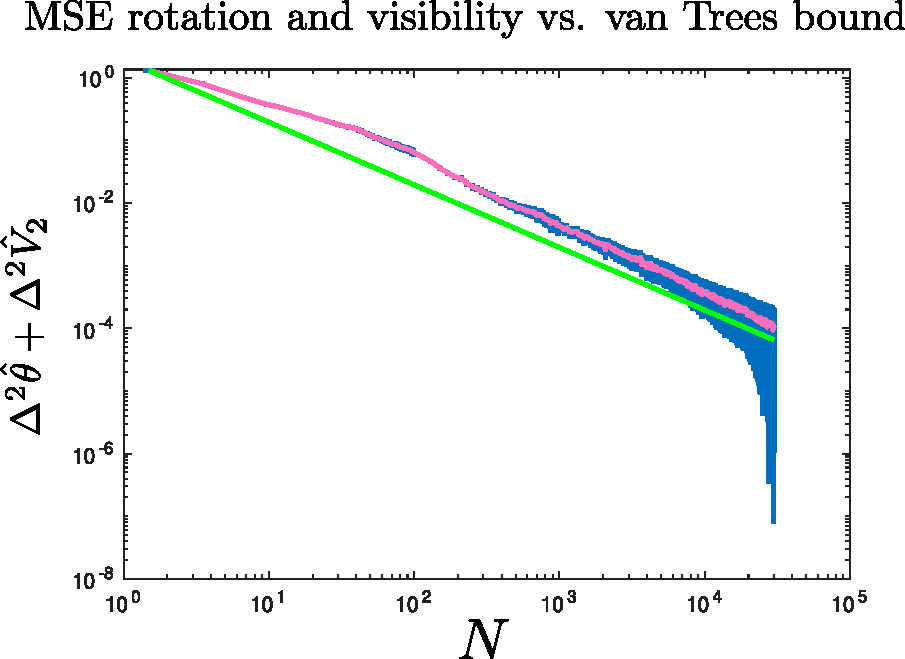
\includegraphics[width=0.5\textwidth]{thetaV2-5000.pdf}
	\end{center}
	\caption{Estimation of the rotation angle and the second visibility (for the stage $s=2$) in which the other visibilities are considered as nuisance parameters performed with $n_p = 5000$. The weight matrix has $G_{11} = 1$ and $G_{33} = 1$ as only non-null entries. The purple line is the precision of the estimation. In blue we plot the error bars.}
	\label{fig:thetaV2-5000}
\end{figure}

\section{Conclusions}
%
Only in Fig.~\ref{fig:theta} the improved quantum scaling seems to be significant. In the other plots traces of a sub-SQL coming from the Heisenberg limited estimation of the rotation can be assessed. 

\section{Thoughts}

\begin{itemize}
	\item The algorithm was instructed to estimate a rotation angle in $[0, 2 \pi)$, however it received only rotation angles in the interval $[0, \pi)$. This issue should be corrected.
	
	\item Is it correct to use uniform priors for the Bayesian estimations? Normally the advice is to avoid sharp boundaries and hard priors in the Bayesian procedure. However the phase is a periodic variable, and therefore there is no real hard boundary. For the visibilities the hard boundaries in the prior are due to its domain $[0, 1]$ and there is no way to avoid this.
	
	%\item I thought the Bayesian CR bound (van Trees) could have taken automatically into account the fact that we start from a uniform distribution for the phase and visibilities, and that the bound could have been valid also for small values of $N$, but this isn't true. In the previous version of these note I introduced a manual correction of the CR bound
	
	%\begin{equation}
	%\Delta^2 \hat{V}_{CR} \rightarrow \max \Big \lbrace \Delta^2 \hat{V}_{CR}, \frac{1}{12} + \left( 0.5-V \right)^2 \Big \rbrace
	%\end{equation}
	
	\item Instead of computing the non linear program of Eq.~\eqref{eq:semidefinite} we could use the average values of $\nu_i$ used by the actual algorithm for each $N$, in this way we obtain a tighter bound. However a useful bound should not depend from quantities computed from the actual Bayesian estimation.
	
	\item It seems that the precision of the visibilities stops improving after it has reached $1/n_{p}$, then it might be that modifying the hyper-parameters of the Bayesian estimation such precision increases.
	
	\item The error on the y-axis we plot in Sec.~\ref{sec:results} are symmetric, that means the bar correspond to the interval $[\Delta^2 \hat{\theta} - \delta \Delta^2 \hat{\theta}, \Delta^2 \hat{\theta} + \delta \Delta^2 \hat{\theta}]$. The distribution of $\Delta^2 \hat{\theta}$ might however not be symmetric, and it is not. That means the symmetric error bars do not have a physical meaning, they are only there to represent the magnitude of the error. If $\delta \Delta^2 \hat{\theta}$ is very close to $\Delta^2 \hat{\theta}$, then the difference $\Delta^2 \hat{\theta} - \delta \Delta^2 \hat{\theta}$ is very close to zero, even if no experiment had the corresponding precision.
	
\end{itemize}

\section{Advices from Rome}

\begin{itemize}
	\item Plot the median value instead of the mean value
	\item {\color{red}Plot the error on $V$ and on $\theta$ on two different plots.}
	\item Is the error in the plots correct? We should maybe divide by a factor $n$.\\
	\item In order to compute the error on the median a Jackknife could be employed. Similarly in order to enhance the statistics of the Bayesian experiments we could perform a resampling procedure.
	\item For the error we should actually use the internal posterior in the Granade algorithm, with a great number of particles $10000-20000$.
	\item Can we use the Bernstein-von Mises theorem to claim that te CR bound is asymptotically reachable?
	\item Can we modify the B-vM theorem so that the limit is reachable also with adaptively chosen $\nu$?
	
	\item I perform $n$ time the execution of one experiment then i can the the mean square error or the median absolute error, however for the median absolute error I don't have any guarantee, that the CR bound will apply, because I won't be able to say rigorously that the distribution of the asymptotic estimator is Gaussian.
	
	\item To solve the problem of the asymmetric error, we could look into a bootstrap procedure that takes into account an asymmetric confidence interval. Then split every figure into two. By using  bootstrap I use a certified and trusted way of computing the error.
	
	\item A low particle number is not sufficient to estimate with precision two parameter.
	
	\item Perform again the estimations with $n_p = 5000$ and $n = 100$, then use bootstrap to enhance this value (sample with repetition from the $100$ values), and compute asymmetric error. Perform this evaluation directly with the \textbf{experimental data}, so that I don't have to do it again later, and save maximum amount of information.
	
	\item There doesn't seems to be a way to generalize the Bernstein-von Mises theorem and claim rigorously that the asymptotic estimator is Gaussian. 
	
	\item Remove all the reference to the van Trees bound. Instead only talk of a generic Bayesian CR bound, that is
	%
	\begin{equation}
		\mathbb{E}_\theta [ \Delta^2 \hat{\theta} ] \ge \frac{C}{N}
	\end{equation}
	%
	The values of $\frac{1}{J} \sum_{j=1}^{J} \Delta^2 \hat{\theta}_j$ is an approximation of that expectation value.
	
	\item Surely computing the median instead of the mean will reduce the outliers, however we don't really have to hide such extremal cases. We can discuss them without the need of smuggling them under the rug.
	
	\item We could compute an asymmetric confidence interval with the bootstrap feature given by Matlab. The problem is how can we combine the confidence intervals of the different phases. https://stackoverflow.com/questions/19686459/bootstrap-and-asymmetric-ci
	
	\item {\color{red} On a second thought the plots}
	
\end{itemize}

\begin{thebibliography}{100}
	
	\bibitem{Cimini2021} V Cimini \textit{et al.}, \href{http://arxiv.org/abs/2110.02908}{arXiv:2110.02908 (2021).}
	%
	
	\bibitem{Granade2012} C E Granade \textit{et al.} 2012 \href{https://doi.org/10.1088/1367-2630/14/10/103013}{New J. Phys. {\bf 14} 103013}.
	%
	
	%\bibitem{Roccia2018} E Roccia \textit{et al.}, \href{https://www.osapublishing.org/optica/abstract.cfm?uri=optica-5-10-1171}{Optica~{\bf 5}, 1171-1176 (2018).}
	%
	
	\bibitem{Belliardo2020} F Belliardo and V Giovannetti, \href{https://link.aps.org/doi/10.1103/PhysRevA.102.042613}{Phys. Rev. A~{\bf 102}, 042613}.
	%
	

	
\end{thebibliography}

\end{document}